% emphasize-more.tex
% Section 4: What Should Be Emphasized MORE

%%%%%%%%%%%%%%%%%%%%
\section{What Should Be Emphasized MORE}
%%%%%%%%%%%%%%%%%%%%

%%%%%%%%%%%%%%%%%%%%
\begin{frame}{Increase Focus On These Topics}
  \begin{center}
    \textbf{Topics that require human expertise and cannot be outsourced to LLMs.}
  \end{center}
  
  \vspace{0.3cm}
  
  \begin{enumerate}
    \item \textbf{Cost Models} --- How choices affect machine code
    \item \textbf{Compiler Transformations} --- Alias analysis, constant folding, UB exploitation
    \item \textbf{API and Library Design} --- Interface stability, composability
    \item \textbf{Trade-off Reasoning} --- Simplicity vs. power vs. safety
    \item \textbf{Execution Models} --- Translation units, linkage, lifetime
    \item \textbf{Standards Rationale} --- Understanding \textit{why} C23 evolved
  \end{enumerate}
  
  \vspace{0.3cm}
  
  \begin{block}{Key Insight}
    These topics connect code to architecture, history, and engineering judgment.
  \end{block}
  
  % Speaker note: These are areas where experience and deep knowledge matter most
\end{frame}
%%%%%%%%%%%%%%%%%%%%

%%%%%%%%%%%%%%%%%%%%
\begin{frame}[fragile]{Cost Models: \texttt{restrict} and Virtual Dispatch}
  \begin{columns}[T]
    \begin{column}{0.48\textwidth}
      \textbf{The \texttt{restrict} Keyword:}
      \begin{block}{Without \texttt{restrict}}
\begin{verbatim}
void add(int *a, int *b,
         int *c, int n) {
  for (int i = 0; i < n; i++)
    c[i] = a[i] + b[i];
}
// Cannot vectorize
\end{verbatim}
      \end{block}
      With \texttt{restrict}: Compiler \textbf{can} vectorize!
    \end{column}
    \begin{column}{0.48\textwidth}
      \textbf{Virtual Dispatch Cost:}
      \begin{block}{Direct vs. Indirect}
\begin{verbatim}
// C: Direct call
handler(d);  // Inlinable

// Java: vtable lookup
h.handle();  // Indirect
\end{verbatim}
      \end{block}
      
      \textbf{Virtual dispatch:} Load vtable pointer, indirect call, harder to inline.
    \end{column}
  \end{columns}
  
  \vspace{0.3cm}
  
  \textbf{Teaching Point:} Students should understand \textit{when} abstraction costs matter.
  
  % Speaker note: Connect to JIT compilation in Java for optimization
\end{frame}
%%%%%%%%%%%%%%%%%%%%

%%%%%%%%%%%%%%%%%%%%
\begin{frame}[fragile]{Cost Models: Cache-Aware Data Layout}
  \textbf{Data-Oriented Design in C}
  
  \begin{columns}[T]
    \begin{column}{0.48\textwidth}
      \begin{block}{Array of Structs (AoS)}
\begin{verbatim}
struct Entity {
  float x, y, z;    // pos
  float vx, vy, vz; // vel
  float mass;
};
Entity entities[1000];
\end{verbatim}
      \end{block}
      \textbf{Problem:} Cache misses when accessing only positions.
    \end{column}
    \begin{column}{0.48\textwidth}
      \begin{block}{Struct of Arrays (SoA)}
\begin{verbatim}
struct Entities {
  float x[1000];
  float y[1000];
  float z[1000];
  float vx[1000];
  // ...
};
\end{verbatim}
      \end{block}
      \textbf{Benefit:} Better cache utilization for position-only access.
    \end{column}
  \end{columns}
  
  % Speaker note: Essential for game development, scientific computing
\end{frame}
%%%%%%%%%%%%%%%%%%%%

%%%%%%%%%%%%%%%%%%%%
\begin{frame}[fragile]{Compiler Transformations: UB Exploitation}
  \textbf{How Compilers Use Undefined Behavior}
  
  \begin{block}{Example: Null Pointer Check Elimination}
\begin{verbatim}
int *p = get_pointer();
int x = *p;           // Dereference before check
if (p == NULL) {      // Compiler removes this!
    handle_error();   // Dead code
}
\end{verbatim}
  \end{block}
  
  \textbf{Compiler Reasoning:}
  \begin{enumerate}
    \item \texttt{*p} dereferences \texttt{p}
    \item If \texttt{p} were \texttt{NULL}, that would be UB
    \item Program assumes no UB $\Rightarrow$ \texttt{p} cannot be \texttt{NULL}
    \item Therefore, remove the entire \texttt{if} block
  \end{enumerate}
  
  \begin{alertblock}{Teaching Point}
    UB is not ``ignored''---it enables aggressive optimization. Real CVEs result from this!
  \end{alertblock}
  
  % Speaker note: Real CVEs have resulted from this optimization pattern
\end{frame}
%%%%%%%%%%%%%%%%%%%%

%%%%%%%%%%%%%%%%%%%%
\begin{frame}[fragile]{API Design and Execution Models}
  \begin{columns}[T]
    \begin{column}{0.48\textwidth}
      \textbf{POSIX File API Principles:}
      \begin{block}{Example}
\begin{verbatim}
int fd = open("f.txt",
              O_RDONLY);
read(fd, buf, sz);
close(fd);
\end{verbatim}
      \end{block}
      
      \textbf{Design Principles:}
      \begin{itemize}
        \item Handle-based resources
        \item Uniform error signaling
        \item Composability (pipes)
        \item Minimal interface
      \end{itemize}
    \end{column}
    \begin{column}{0.48\textwidth}
      \textbf{Translation Units \& Linkage:}
      \begin{block}{file1.c \& file2.c}
\begin{verbatim}
static int count = 0;
void increment(void) {
  count++;
}
// Both "count" are separate!
\end{verbatim}
      \end{block}
      
      \textbf{Key Concepts:}
      \begin{itemize}
        \item \texttt{static} = internal linkage
        \item No \texttt{static} = external linkage
        \item Linker resolves symbols
      \end{itemize}
    \end{column}
  \end{columns}
  
  % Speaker note: Essential for understanding large C projects like Linux
\end{frame}
%%%%%%%%%%%%%%%%%%%%

%%%%%%%%%%%%%%%%%%%%
\begin{frame}{Trade-offs and Standards Evolution}
  \begin{columns}[T]
    \begin{column}{0.48\textwidth}
      \textbf{Safety vs. Performance:}
      \begin{center}
        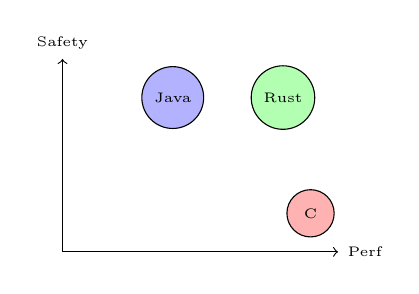
\begin{tikzpicture}[scale=0.7]
          \draw[->] (0,0) -- (5,0) node[right] {\tiny Perf};
          \draw[->] (0,0) -- (0,3.5) node[above] {\tiny Safety};
          \node[draw, circle, fill=red!30, minimum size=0.6cm] at (4.5,0.7) {\tiny C};
          \node[draw, circle, fill=blue!30, minimum size=0.6cm] at (2,2.8) {\tiny Java};
          \node[draw, circle, fill=green!30, minimum size=0.6cm] at (4,2.8) {\tiny Rust};
        \end{tikzpicture}
      \end{center}
      
      Every language makes trade-offs. Students must understand \textit{which} and \textit{why}.
    \end{column}
    \begin{column}{0.48\textwidth}
      \textbf{Why C23 Matters:}
      
      \textbf{Key Changes:}
      \begin{itemize}
        \item \texttt{nullptr} keyword
        \item \texttt{typeof} operator
        \item \texttt{\#embed} directive
        \item Removal of K\&R decls
      \end{itemize}
      
      \textbf{Why?}
      \begin{itemize}
        \item Type safety
        \item Security hardening
        \item C++ compatibility
      \end{itemize}
    \end{column}
  \end{columns}
  
  \vspace{0.2cm}
  
  \textbf{Reference:} ACM Queue ``Catch-23: The New C Standard'' (2023)
  
  % Speaker note: Standards evolution reflects lessons learned
\end{frame}
%%%%%%%%%%%%%%%%%%%%
